\section{Auswertung}

\subsection{Strom-Spannungs-Kennlinie}
\label{kap:Kennlinie}
Für eine effiziente Detektion von Strahlung muss der Sensor vollständig depletiert sein. Zur Abschätzung der Depletionsspannung des verwendeten Streifendetektors wird eine Strom-Spannungs-Kennlinie aufgenommen. Die ermittelten Messwerte des Leckstromes $I$ und der Spannung $U$ sind Tabelle \ref{tab:UI-Kennlinie} zu entnehmen. Es wurden zwei Messreihen aufgenommen, da im Laufe der Versuchsdurchführung aufgefallen ist, dass der maximal angelegte Spannungswert möglicherweise zu niedrig gewählt wurde. Um diese Vermutung zu überprüfen, wurde zu diesem Zeitpunkt die zweite Messung durchgeführt.

\begin{table}[ht]
  \centering
  \caption{Messwerte des Leckstromes $I$ in Abhängigkeit der angelegten Vorspannung $U$ für zwei Messungen.}
  \label{tab:UI-Kennlinie}
  \sisetup{table-format=2.1}
  \begin{tabular} { c c c | c c c}
  \toprule
  {$U$ /[V]} & {$I_1$ [$\mu$A]} & {$I_2$ [$\mu$A]} & {$U$ /[V]} & {$I_1$ [$\mu$A]} & {$I_2$ [$\mu$A]}\\
  \midrule
     0 & 0.76 & 0.78 & 110& 0.96 & 1.05 \\
    10 & 0.78 & 0.81 &  120& 0.96 & 1.05\\
    20 & 0.80 & 0.85 &  130& 0.97 & 1.06\\
    30 & 0.83 & 0.91 &  140& & 1.06 \\
    40 & 0.87 & 0.96 &  150& & 1.06 \\
    50 & 0.90 & 0.99 &  160& & 1.07 \\
    60 & 0.93 & 1.01 &  170& & 1.07 \\
    70 & 0.93 & 1.02 &  180& & 1.08 \\
    80 & 0.94 & 1.03 &  190& & 1.08 \\
    90 & 0.95 & 1.03 &  200& & 1.08 \\
    100& 0.95 & 1.04 \\
  \bottomrule
  \end{tabular}
  \end{table}
  \FloatBarrier

  Die Messwerte sind in Abbildung \ref{fig:UI-Kennlinie} graphisch dargestellt.
  Nähert sich die angelegte Spannung $U$ der Depletionsspannung $U_\mathrm{Dep}$, geht die Kennlinie in einen linearen Sättigungsverlauf über. In diesem Bereich tragen lediglich Exzitonen aus thermischen Anregungen zum Leckstrom bei, da die ladungsträgerarme Zone über den gesamten Sensor ausgebreitet ist. Bei Spannungen unterhalb von $U_\mathrm{Dep}$ tragen zusätzlich freie Ladungsträger der Dotierungen zum Leckstrom bei. In diesem Übergang wird die Depletionsspannung auf einen Wert von
  \begin{align*}
    U_\mathrm{Dep} \approx \SI{61}{\volt}
  \end{align*}
  abgeschätzt. Im weiteren Verlauf wird die Vorspannung auf einen Wert von $U=\SI{85}{\volt}$ geregelt.

\begin{figure}
  \centering
  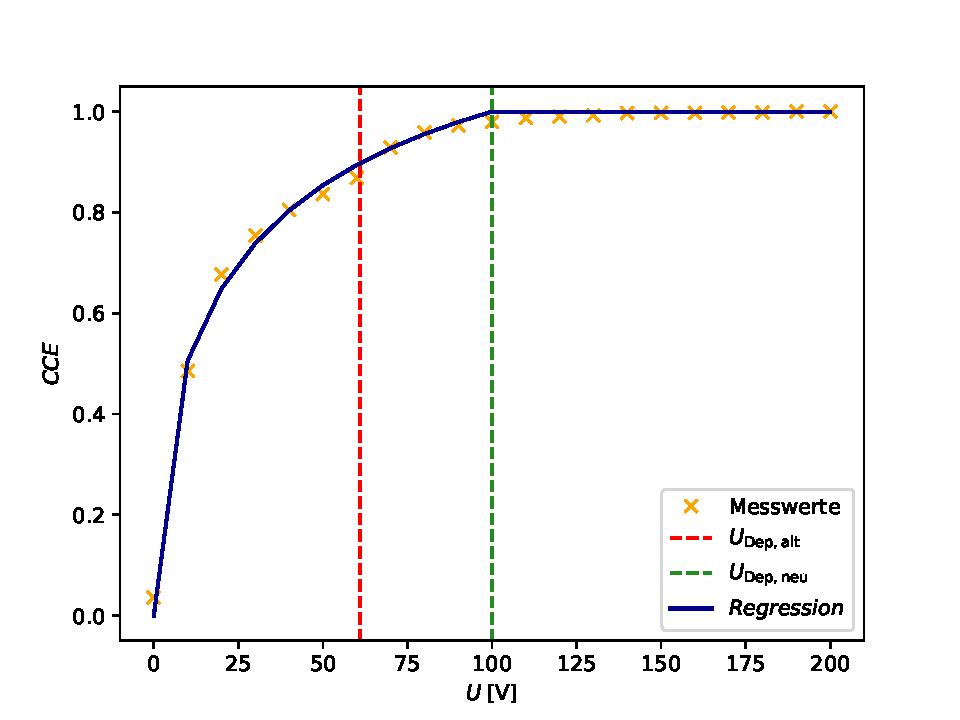
\includegraphics[width=0.8\textwidth]{plots/Kennlinie_Laser.pdf}
  \caption{Leckstrom $I$ in Abhängigkeit der angelegten Spannung $U$ für zwei Messreihen. Im Beginn des Plateus findet sich die abgeschätzte Depletionsspannung $U_\mathrm{Dep}$.}
  \label{fig:UI-Kennlinie}
\end{figure}
\FloatBarrier

\subsection{Pedestals und Noise}
\label{kap:Pedestal}
Durch verschiedene Störquellen enthält das vom Detektor empfangene Signal ein Rauschen. Zum Abschätzen des Untergrundes wird eine Messung ohne externe Quellen durchgeführt, sodass lediglich das Rauschsignal vom Sensor detektiert wird. Aus den gemessenen Signalen werden anschließend nach Gleichungen \eqref{eq:15} und \eqref{eq:16} die Pedestal- sowie die Noisewerte berechnet und in Abbildung \ref{fig:Pedestals} in Abhängigkeit von der Streifennummer aufgetragen.
\begin{figure}
  \centering
  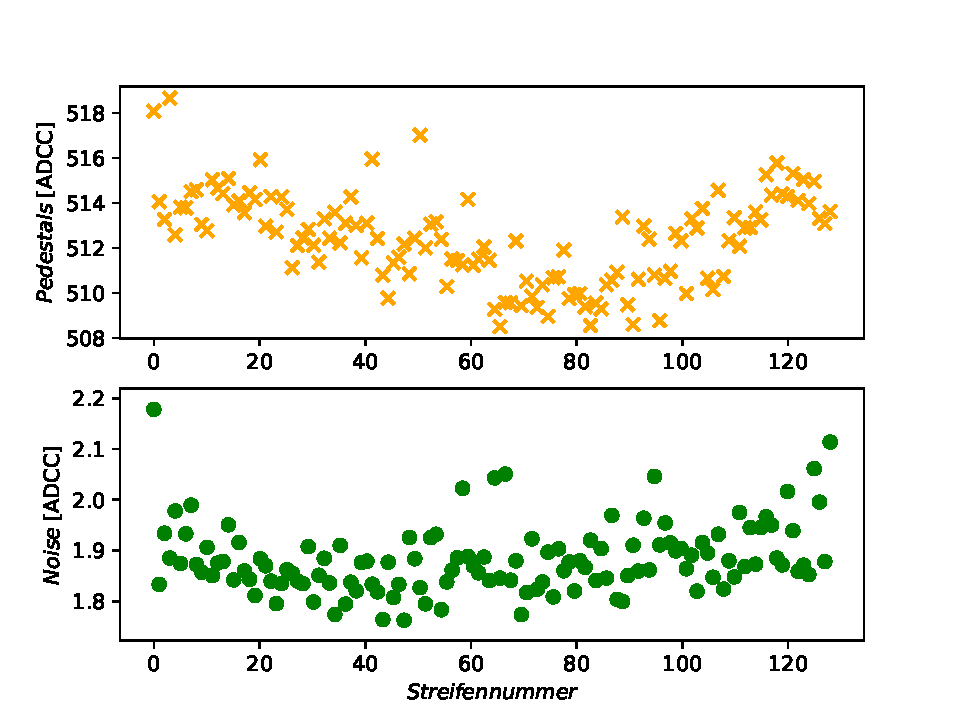
\includegraphics[width=0.8\textwidth]{plots/Pedestals_Noise.pdf}
  \caption{Darstellung der berechneten Pedestal- und Noisewerte in Abhängigkeit von der Streifennummer.}
  \label{fig:Pedestals}
\end{figure}
\FloatBarrier
Die Pedestals weisen eine Schwankung um etwa 10 ADCC auf. Bei den Streifennummern 60 bis 100 fallen hierbei besonders niedrige Pedestalwerte ins Auge.
Über alle Kanalnummern hinweg ist ein regelmäßiges Rauschsignal von bis zu 0.3 ADCC zu beobachten.

Des Weiteren werden die Werte des Common-Mode-Shifts mittels Gleichung \eqref{eq:18} berechnet. Die Verteilung der Werte ist in Abbildung \ref{fig:CommonModeShift} dargestellt. Da nach \cite{anleitung} eine Gaußverteilung der Werte um Null zu erwarten ist, wird die Varianz der Common-Mode-Shift-Verteilung ermittelt und eine entsprechende Gaußkurve in die Werte gelegt.
\begin{figure}
  \centering
  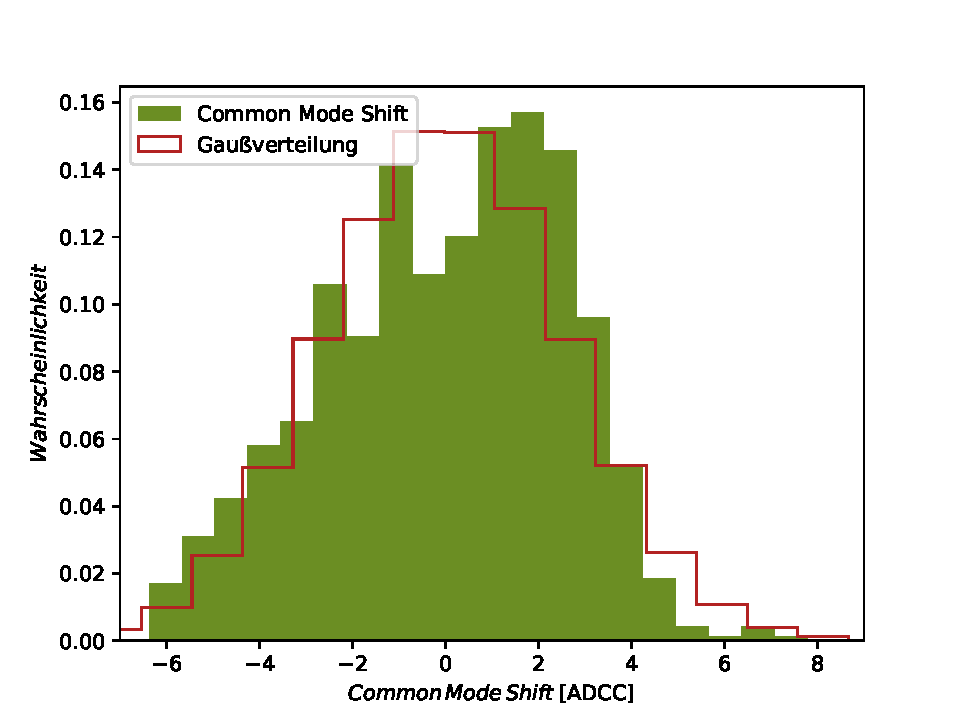
\includegraphics[width=0.8\textwidth]{plots/CommonModeShift.pdf}
  \caption{Verteilung der berechneten Common-Mode-Shift-Werte und die zu erwartende Gaußverteilung um Null.}
  \label{fig:CommonModeShift}
\end{figure}
\FloatBarrier
Im Vergleich der Common-Mode-Shift-Verteilung mit der zu erwartenden Gaußverteilung ist eine Verschiebung des Wahrscheinlichkeitsmaximums des Common-Mode-Shifts zu höhreren Werten hin zu erkennen. Außerdem steigt die Verteilung flacher an und fällt rascher ab, als die Gaußkurve.

Eine Korrektur des Untergrundes wird im Folgenden elektronisch durch ein \textit{python}-Skript durchgeführt, auf welches hier nicht weiter eingegangen wird.

\subsection{Kalibration}
\label{kap:Kalibration}
Um aus den gemessenen ADCC einen Wert für die im Detektor deponierte Energie zu erhalten, ist eine Kalibrationsmessung nötig. Hierzu werden fest definierte Elektronenpulse an den Detektor gesendet und die jeweiligen ADCC aufgenommen.
Durch die Zuleitungen entstehen Verzögerungen der Signale. Um Fehlerquellen diesbezüglich zu vermeiden, wird zunächst eine optimale Verzögerungszeit zwischen dem gesendeten Puls und der Auslese der Sensoren ermittelt. Zu diesem Zweck werden die ADCC in Abhängigkeit von der Verzögerungszeit aufgenommen, welche in Abbildung \ref{fig:Delay} zu erkennen sind. Die optimale Verzögerungszeit lässt sich an der Stelle ausmachen, wo eine maximale Anzahl an ADCC registriert wird. Dieses ist bei einem Zeitabstand von $t_\mathrm{Delay}=\SI{61}{\nano\second}$ der Fall.
\begin{figure}
  \centering
  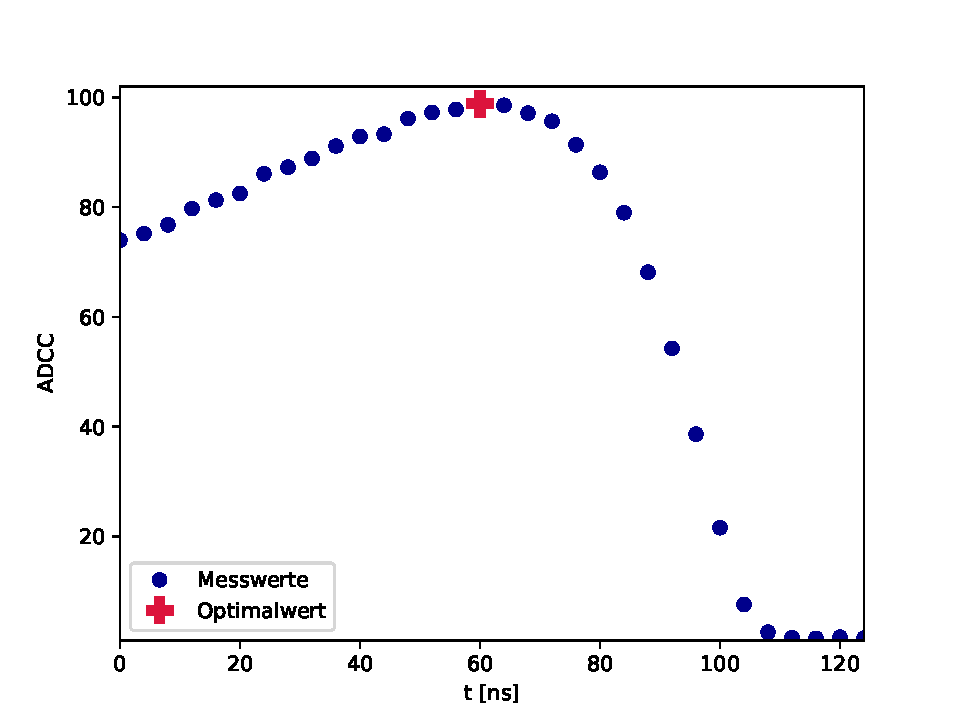
\includegraphics[width=0.8\textwidth]{plots/Delay.pdf}
  \caption{ADCC in Abhängigkeit von der Verzögerungszeit zwischen gesendeten Elektronenpuls und Auslese der Sensoren. Die optimale Verzögerungszeit (rotes Kreuz) ist im Maximum der ADCC zu finden.}
  \label{fig:Delay}
\end{figure}
\FloatBarrier
Die Messdaten des \textit{Calibration Run} bei einer angelegten Spannung von $U=U_\text{Dep}$, nämlich die ADCC für den jeweiligen Elektronenpuls, sind für vier verschiedene Streifen mit den Streifennummern 50, 70, 80 und 90 in Abbildung \ref{fig:KanalPlot} zu erkennen. Zum Abschätzen der Energie, welche durch die Elektronen auf den Sensor auftrifft, wird die Anzahl der gesendeten Elektronen mit der Energie, welche zur Erzeugung eines Elektronen-Loch-Paares in Silizium ($\SI{3.6}{\electronvolt}$) nötig ist, multipliziert. Zusätzlich sind diese Wertepaare in Abbildung \ref{fig:0V80V} für einen weiteren Streifen mit der Streifennummer 60 bei Vorspannungen von $U=\SI{0}{\volt}$ und $U=U_\mathrm{Dep}$ zum Vergleich dargestellt.
\begin{figure}
  \centering
  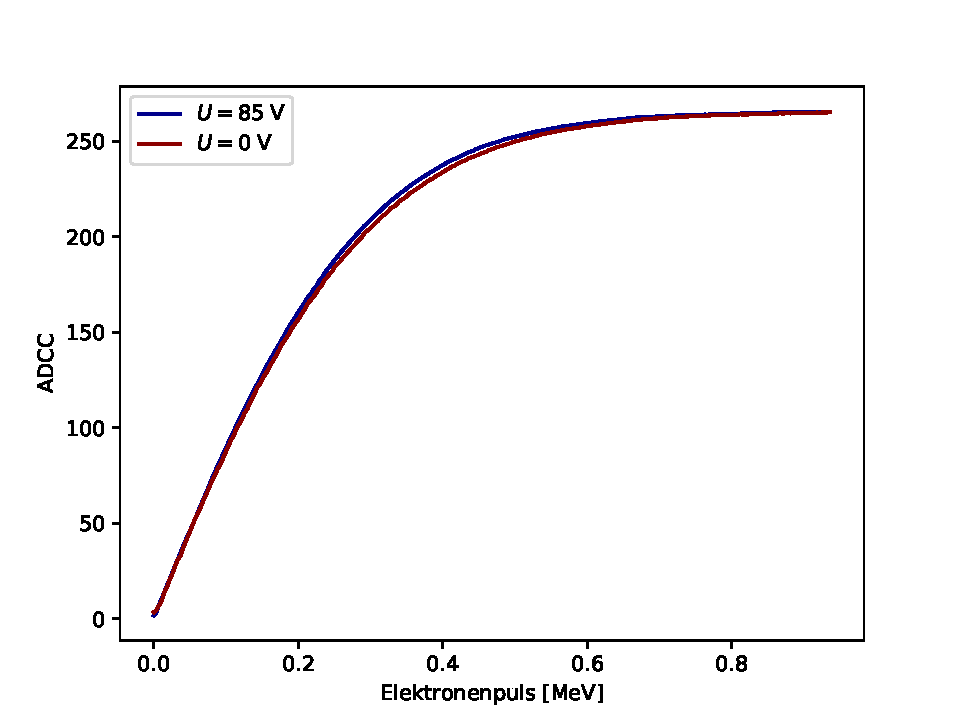
\includegraphics[width=0.8\textwidth]{plots/0V_80V_Vergleich.pdf}
  \caption{ADCC des \textit{Calibration Run} in Abhängigkeit des Elektronenpulses für eine angelegte Spannung von $U=\SI{0}{\volt}$ und $U=U_\mathrm{Dep}$ des Streifen 60.}
  \label{fig:0V80V}
\end{figure}
\FloatBarrier
\begin{figure}
  \centering
  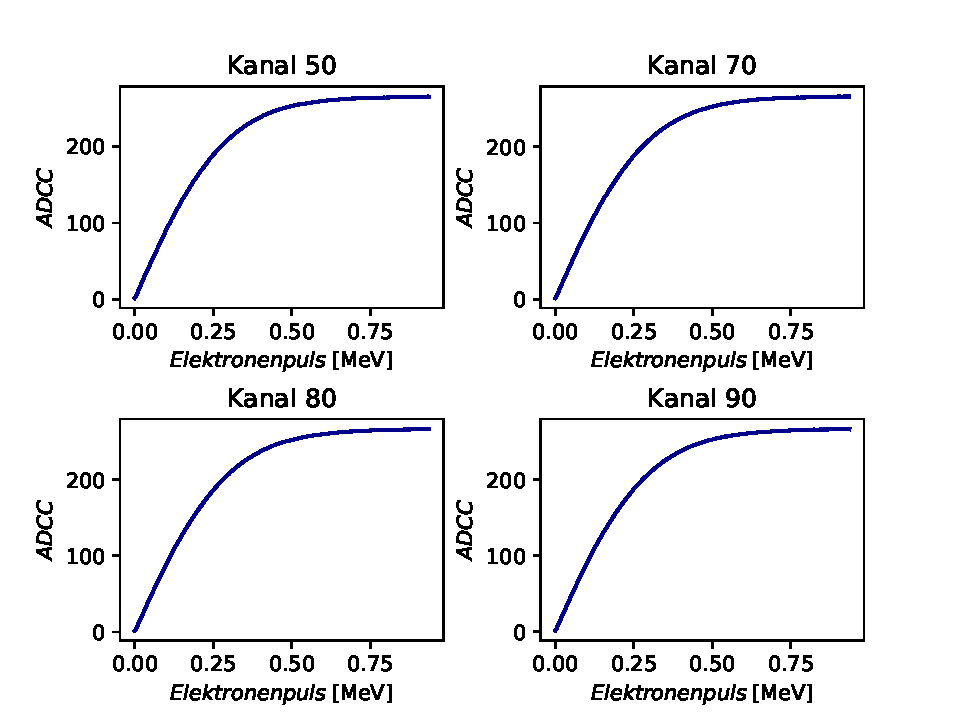
\includegraphics[width=0.8\textwidth]{plots/Kalib_Kanal_Plot.pdf}
  \caption{ADCC des \textit{Calibration Run} in Abhängigkeit des Elektronenpulses für die Streifen 50, 70, 80 und 90.}
  \label{fig:KanalPlot}
\end{figure}
\FloatBarrier
Alle Kurven steigen zunächst an und gehen ab einen Elektronenpuls von etwa $\SI{0.5}{\electronvolt}$ in einen Sättigungsverlauf über. Der Sensor scheint somit lediglich im Bereich unterhalb $\SI{0.5}{\electronvolt}$ eine sinnvolle Energieauflösung zu haben.
Die einzelnen Kurven weisen kaum Abweichungen untereinander auf. Auch der Vergleich der ADCC-Verläufe bei unterschiedlichen Spannungen zeigt kaum Unterschiede. Es kann somit davon ausgegangen werden, dass die Kalibration unabhängig von der Vorspannung durchgeführt werden kann.

Zum Finden der Umrechnungsfunktion zwischen ADCC und eintreffender Energie wird der Mittelwert der ADCC für einen festen Elektronenpuls über die fünf vermessenen Streifen ermittelt. Aufgrund der geringen Abweichungen der ADCC-Verläufe in den verschiedenen Kanälen wird der Fehler des Mittelwertes im Folgenden vernachlässigt. In Abbildung \ref{fig:Regression} sind die Energien der gesendeten Elektronenpulse gegen diese Mittelwerte aufgetragen. Zum Ermitteln des Zusammenhanges zwischen ADCC und Puls wird eine Regressionsrechnung durchgeführt. Ausgegangen wird hierbei von einem Polynom vierten Gerades der Form
\begin{align}
  Q(ADCC) = a\,ADCC^4 + b\,ADCC^3 + c\,ADCC^2 + d\,ADCC + e.
  \label{eq:Kalib}
\end{align}
In die Rechnung werden lediglich die Werte aus dem Bereich eingebunden, in dem ein direkter Zusammenhang der Größen ersichtlich ist. Im darauffolgenden Bereich knickt der Kurvenverlauf ab und scheint gegen einen unendlich hohen Wert zu streben. Hier ist eine eindeutige Zuweisung eines ADCC-Werts zu einem einzigen Pulswert nicht mehr möglich.
Für die Parameter der Umrechnungsfunktion ergeben sich mittels \textit{curve\_fit} des Paketes \textit{scipy.optimize} die Werte
\begin{align*}
  a &= \SI{178 (8)e-6}{\electronvolt},\\
  b &= (-0.059 \pm 0.004) \; \si{\electronvolt},\\
  c &= \SI{79(7)}{\electronvolt},\\
  d &= \SI{736(45)}{\electronvolt},\\
  e &= \SI{2534(815)}{\electronvolt}.
\end{align*}

\begin{figure}
  \centering
  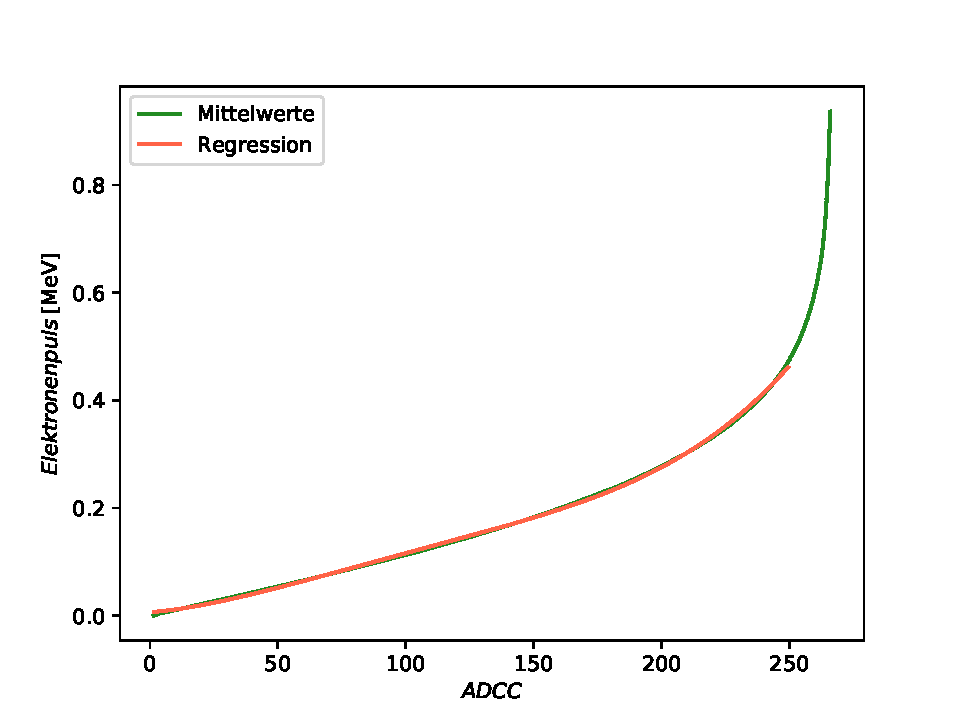
\includegraphics[width=0.8\textwidth]{plots/Kalibrationsregression.pdf}
  \caption{Darstellung der Werte der dem Detektor zugeführten Energie in Abhängigkeit der gemessenen ADCC mit der Regressionsfunktion zur Umrechnung eines ADCC in einen Energiewert.}
  \label{fig:Regression}
\end{figure}
\FloatBarrier

\subsection{Vermessung der Sensoren mittels Laser}
\label{kap:Vermessung}
Für das Durchführen von Messungen mit einer Laserquelle muss die Laserposition sehr genau justiert werden, da dieser nur eine sehr kleine Strahlausdehnung besitzt. Aus diesem Grund muss der Laser so ausgerichtet werden, dass er genau einen Streifen trifft, wofür die Position der Steifensensoren bekannt sein muss. Hierzu wird das Signal für verschiedene Laserpositionen aufgenommen.

Zunächst muss erneut die optimale Verzögerungszeit zwischen Laserimpuls und Auslese ermittelt werden. Das Vorgehen erfolgt analog zum vorherigen Abschnitt \ref{kap:Kalibration}. Aus den Messwerten, welche Abbildung \ref{fig:Delay Laser} zu entnehmen sind, ergibt sich eine optimale Verzögerungszeit von $t_\mathrm{Delay}=\SI{108}{\nano\second}$.
\begin{figure}
  \centering
  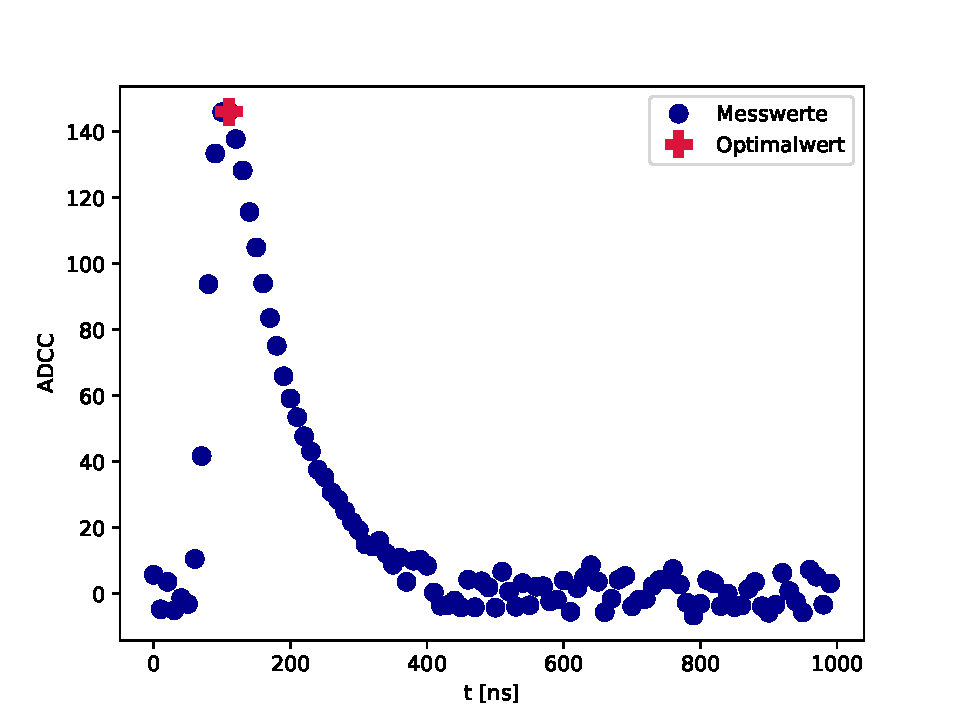
\includegraphics[width=0.8\textwidth]{plots/Delay_Laser.pdf}
  \caption{ADCC in Abhängigkeit von der Verzögerungszeit zwischen Laserpuls und Auslese der Sensoren. Die optimale Verzögerungszeit (rotes Kreuz) ist im Maximum der ADCC zu finden..}
  \label{fig:Delay Laser}
\end{figure}
\FloatBarrier
Um die Streifen zu ermitteln, welche vom Laser getroffen werden, wird die Intensität des Signales eines jeden Kanales in Abhängigkeit von der Laserposition in Abbildung \ref{fig:Position} dargestellt. Die Signalintensität wird in dieser Abbildung als Kreisgröße dargestellt, wobei ein größerer Kreis einem höheren Signal entspricht. Die Laserposition null entspricht hierbei der Startposition.
\begin{figure}
  \centering
  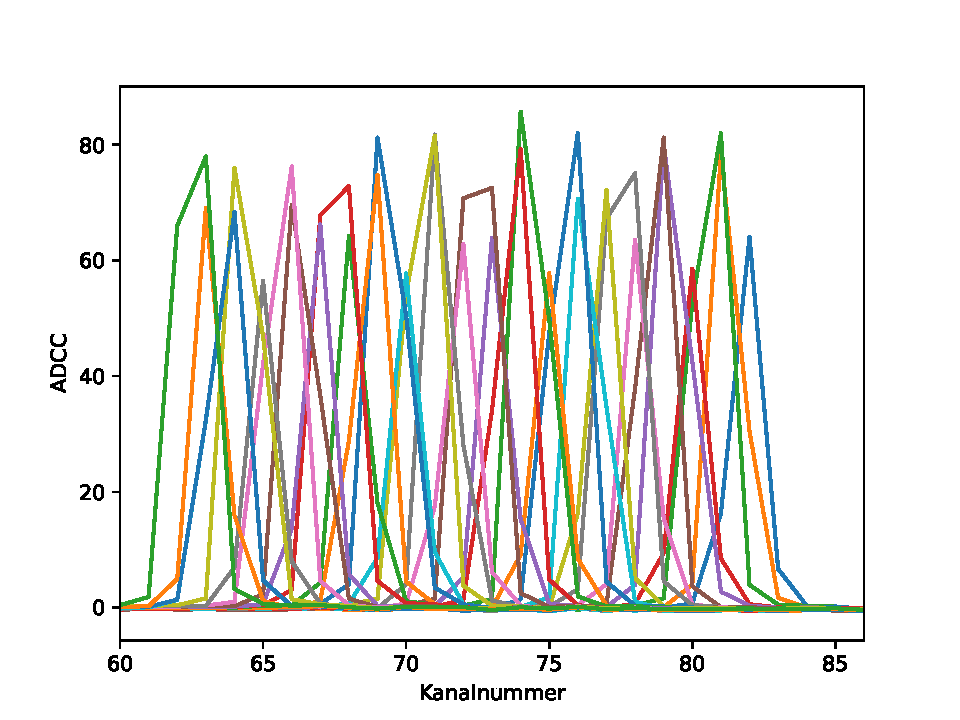
\includegraphics[width=0.8\textwidth]{plots/Position_Kanal_Signal_Plot.pdf}
  \caption{Darstellung der ADCC für jeden Kanal in Abhängigkeit von der Laserposition. Ein größerer Kreis entspricht hierbei einer höheren Anzahl an ADCC.}
  \label{fig:Position}
\end{figure}
\FloatBarrier
Es ist eindeutig zu erkennen, dass die Kanalnummern 61 bis 81 von dem Laser getroffen werden.

Der Abstand der Streifensensoren, auch \textit{pitch} genannt, kann über den Abstand der Signalmaxima zweier benachbarter Streifen ermittelt werden. Diese entstehen immer dann, wenn der Laser genau auf einen Sensor trifft. Für jeden Kanal der Nummern 61 bis 81 wird daher die Laserposition ermittelt, für die das Signal einen maximalen Wert annimmt. Diese Maximapositionen sind für jeden Kanal in Abbildung \ref{fig:Maxima} dargestellt.
\begin{figure}
  \centering
  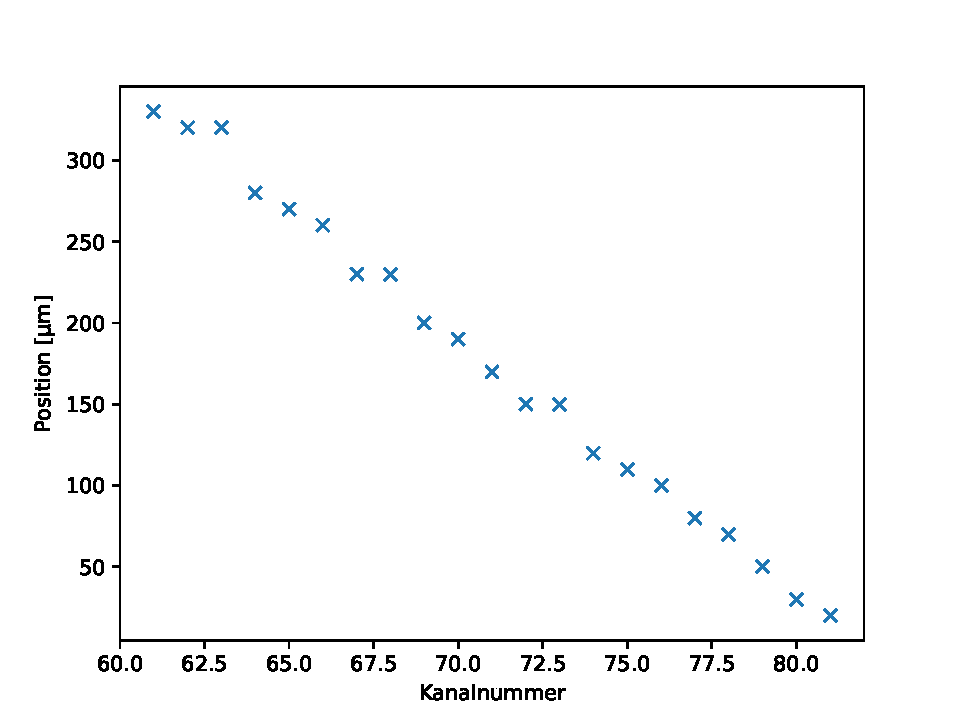
\includegraphics[width=0.8\textwidth]{plots/Maxima.pdf}
  \caption{Position des Lasers, an der eine maximale Anzahl an ADCC gemessen wird in Abhängigkeit von der Kanalnummer.}
  \label{fig:Maxima}
\end{figure}
\FloatBarrier
Für jeden Streifen wird anschließend der Abstand der Maximumposition zur Maximumposition des benachbarten Streifen ermittelt und anschließend der Mittelwert der Abstände gebildet.
Somit kann die \textit{pitch} $p$ der Streifen zu
\begin{align*}
  b = \SI{15(2)}{\micro\metre}
\end{align*}
bestimmt werden.
Solange der Laser einen Streifen trifft, wird ein Signal in diesem registriert. Über die Differenz der Maximumsposition zu der Position, an welcher das erste bzw. letzte Signal im Streifen zu erkennen ist, kann daher die Ausdehnung des Lasers auf dem Sensor ermittelt werden. Hierzu wird jeweils die Länge der ansteigenden und abfallenden Flanken jeder Kanalnummer bestimmt und anschließend über alle Flankenlängen gemittelt. Berücksichtigt werden hierbei Signale, deren ADCC größer als 1 sind. Es ergibt sich eine Laserausdehnung $d$ von
\begin{align*}
  d = \SI{292(17)}{\micro\metre}.
\end{align*}

\subsection{Bestimmung der CCE mittels Laser}
\label{kap:CCEL}
In diesem Abschnitt wird die Ladungsansammlungseffizienz, CCE, bei Bestrahlung mit einem Laser untersucht. Der Laser wurde hierfür so positioniert, dass ein Signalmaximum zu beobachten ist. Die Position entspricht der Laserposition von $\SI{320}{\micro\metre}$. Mit Hilfe von Abbildung \ref{fig:Position} wird ersichtlich, dass in dieser Position der Streifen 62 vom Laser getroffen wird.

Die in Kanal 62 aufgenommenen spannungsabhängigen ADCC werden auf den Sättigungswert normiert und in Abbildung \ref{fig:KennlinieLaser} gegen die angelegte Spannung aufgetragen. Es ergibt sich der bekannte Kennlinienverlauf. Im Übergang der Werte in den Sättigungsbereich kann erneut die Depletionsspannung abgeschätzt werden. Zum Vergleich ist in Abbildung \ref{fig:KennlinieLaser} die im Kapitel \ref{kap:Kennlinie} bestimmte Depletionsspannung dargestellt.
\begin{figure}
  \centering
  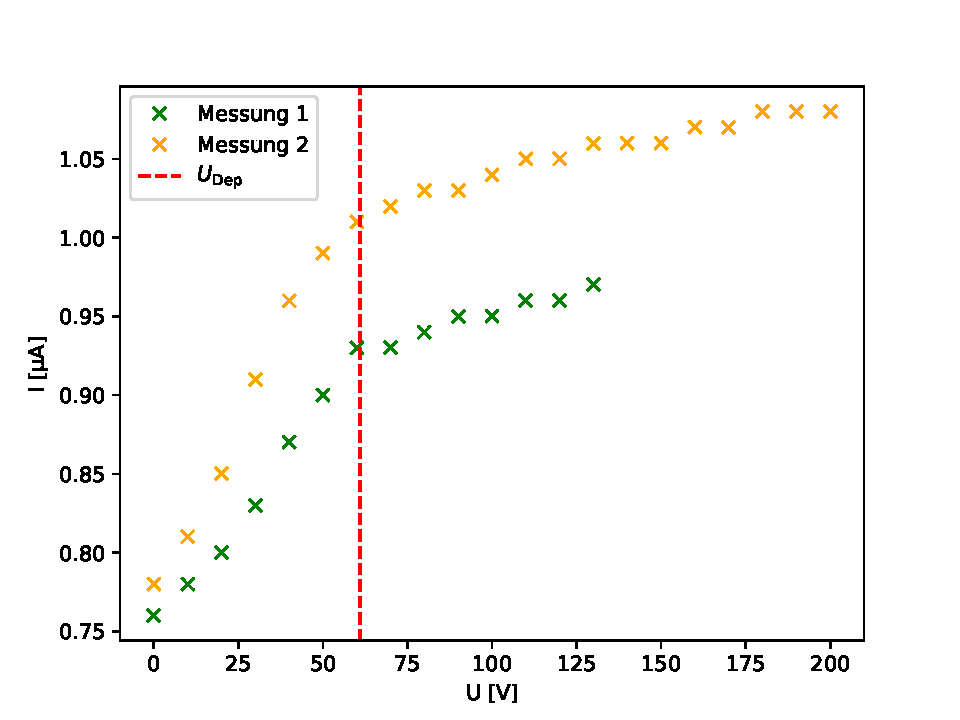
\includegraphics[width=0.8\textwidth]{plots/Kennlinie.pdf}
  \caption{In Gelb sind die Messwerte der ADCC in Abhängigkeit von der Vorspannung, in rot die bestimmte Depletionsspannung aus Kapitel \ref{kap:Kennlinie} und in blau die Regressionsfunktion zur Berechnung der Lasereindringtiefe zu erkennen.}
  \label{fig:KennlinieLaser}
\end{figure}
\FloatBarrier
Die Eindringtiefe des Lasers kann über eine Regressionsrechnung von Gleichung \eqref{eq:20} aus den Kennlinienwerten berechnet werden. Mittels der Funktion \textit{curve\_fit} von \textit{scipy.optimize} wird für die Eindringtiefe ein Wert von
\begin{align*}
   a= \SI{565(218)}{\micro\metre}
\end{align*}
ermittelt.

\subsection{Bestimmung der CCE mittels $^{90}$Sr-Quelle}
Zur Bestimmung der CCE unter Bestrahlung des Sensors mit einer $^{90}$Sr-Quelle werden erneut die ADCC in Abhängigkeit von der angelegten Spannung aufgenommen. Für jeden Spannungswert werden die ADCC eines einzelnen Clusters addiert und anschließend der Mittelwert der addierten ADCC über alle Cluster gebildet. Diese sind, auf den Sättigungswert normiert, in Abbildung \ref{fig:KennlinieQuelle} gegen die Vorspannung aufgetragen. Zusätzlich sind die Effizienzwerte aus der Lasermessung zum Vergleich dargestellt.
\label{kap:CCEQ}
\begin{figure}
  \centering
  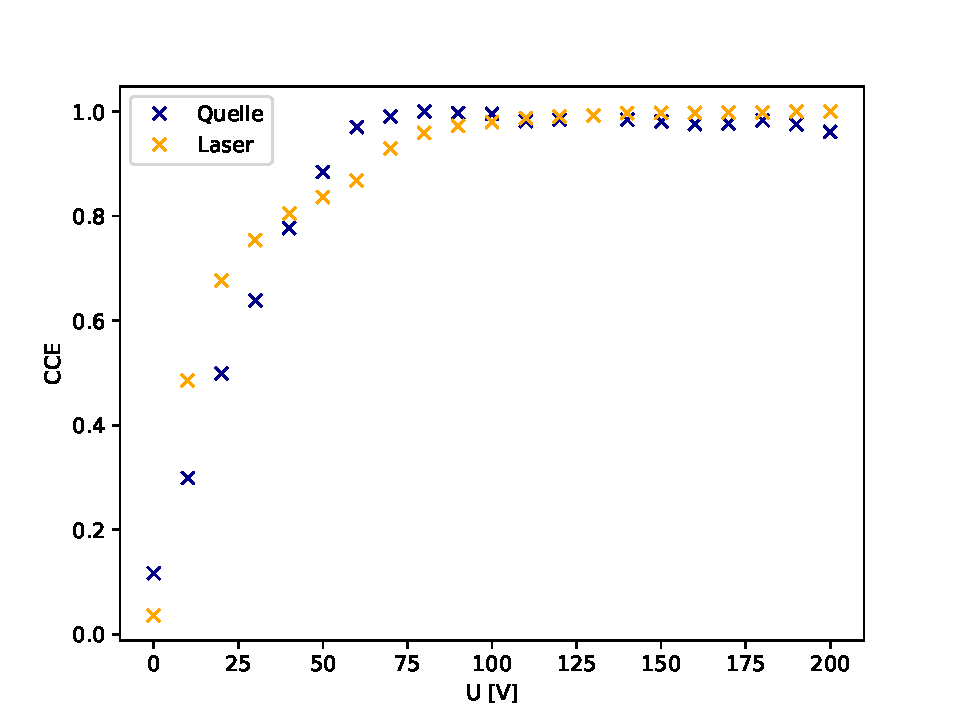
\includegraphics[width=0.8\textwidth]{plots/Effizienz.pdf}
  \caption{Darstellung der auf den Sättigungswert normierten ADCC unter Bestrahlung mit einer $^{90}$Sr-Quelle und einem Laser in Abhängigkeit der Vorspannung.}
  \label{fig:KennlinieQuelle}
\end{figure}
\FloatBarrier
Die CCE-Werte des Lasers weisen einen schnelleren Anstieg auf und gehen etwas früher in den Sättigungsverlauf über. Der Übergang der Quellenkennlinie ist hierbei kürzer, sodass beide Kennlinien den Sättigungswert in etwa gleichzeitig erreichen. Auffällig ist, dass die CCE-Werte der Quelle bei hohen Spannungen wieder leicht abnehmen.

\subsection{Energiespektrum einer $^{90}$Sr-Quelle}
\label{kap:Quelle}
Zuletzt wird das Energiespektrum einer $^{90}$Sr-Quelle aufgenommen.

Zunächst werden die generierten Cluster ausgewertet. In Abbildung \ref{fig:cluster} ist die Verteilung der Clustergröße, sowie der Anzahl an Cluster pro Event graphisch dargestellt. Die Clustergröße repräsentiert hierbei die Anzahl an Kanälen, welche einem Cluster zugeordnet werden.
Es ist ersichtlich, dass eine Bildung von einem Cluster pro Event am wahrscheinlichsten ist. Maximalwert liegt bei fünf Clustern pro Event, welcher aber nur sehr selten erreicht wird.
Ein Cluster besteht zumeist aus einer geringen Anzahl von ein bis zwei Streifen. Der größte generierte Cluster umfasst 15 Streifen.
\begin{figure}
  \centering
  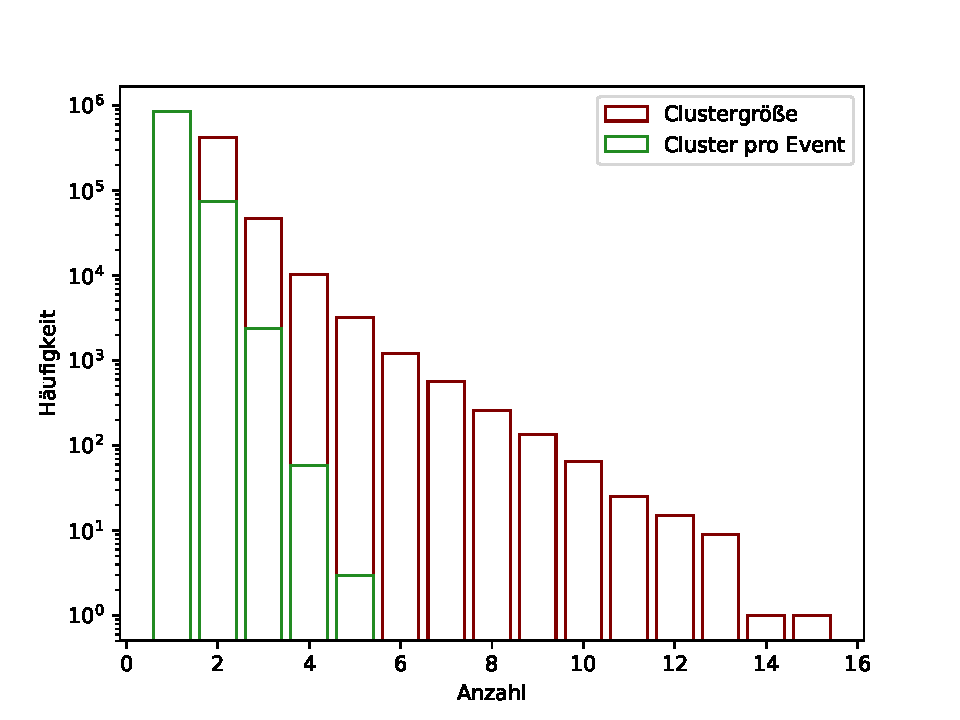
\includegraphics[width=0.8\textwidth]{plots/Cluster.pdf}
  \caption{Häufigkeit der Anzahl der an einem Cluster beteiligten Streifen (Clustergröße) und der Anzahl an Clustern pro Event.}
  \label{fig:cluster}
\end{figure}
\FloatBarrier
In Abbildung \ref{fig:hitmap} ist die Hitmap dargestellt, welche der Verteilung der registrierten Ereignisse auf die Streifen entspricht. Um die Streifennummer 70 herum ist ein breites Maximum der Verteilung auszumachen. Im Vergleich mit der Signalverteilung der Lasermessung sind deutlich mehr Streifen an der Detektion eines Events beteiligt. Dieses lässt auf die größere Strahlausdehnung der Quelle schließen.
\begin{figure}
  \centering
  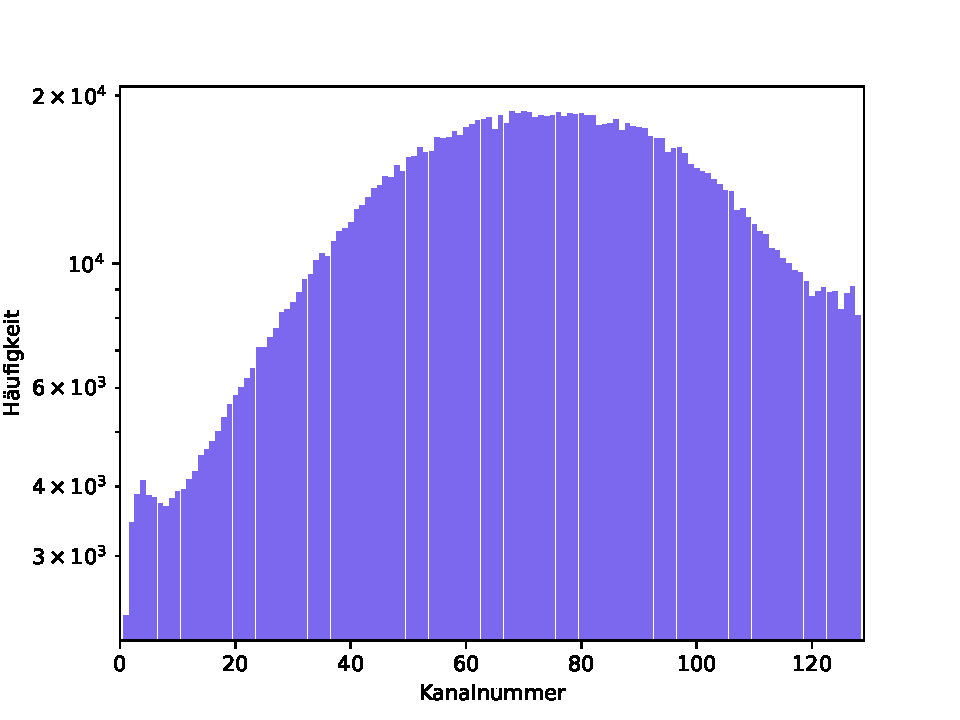
\includegraphics[width=0.8\textwidth]{plots/hitmap.pdf}
  \caption{Darstellung der Häufigkeit der Detektion eines Ereignisses in den einzelnen Streifen (Hitmap).}
  \label{fig:hitmap}
\end{figure}
\FloatBarrier
Um das Energiespektrum zu erhalten, werden die ADCC mit Hilfe der Kalibrierungsfunktion \eqref{eq:Kalib} in Energiewerte umgerechnet und für die einzelnen Cluster addiert. Da die Umrechnungsfunktion lediglich bis zu einem ADCC-Wert von etwa 240 gültig ist, werden Messwerte oberhalb dieser Grenze nicht weiter beachtet.
Zusätzlich wird das Spektrum der ADCC dargestellt, wozu die Einträge pro Cluster lediglich addiert werden.
Die Verteilungen sind in Abbildung \ref{fig:spektrumADCC} für die ADCC und in Abbildung \ref{fig:spektrumkeV} für die Energiewerte dargestellt.

\begin{figure}
  \centering
  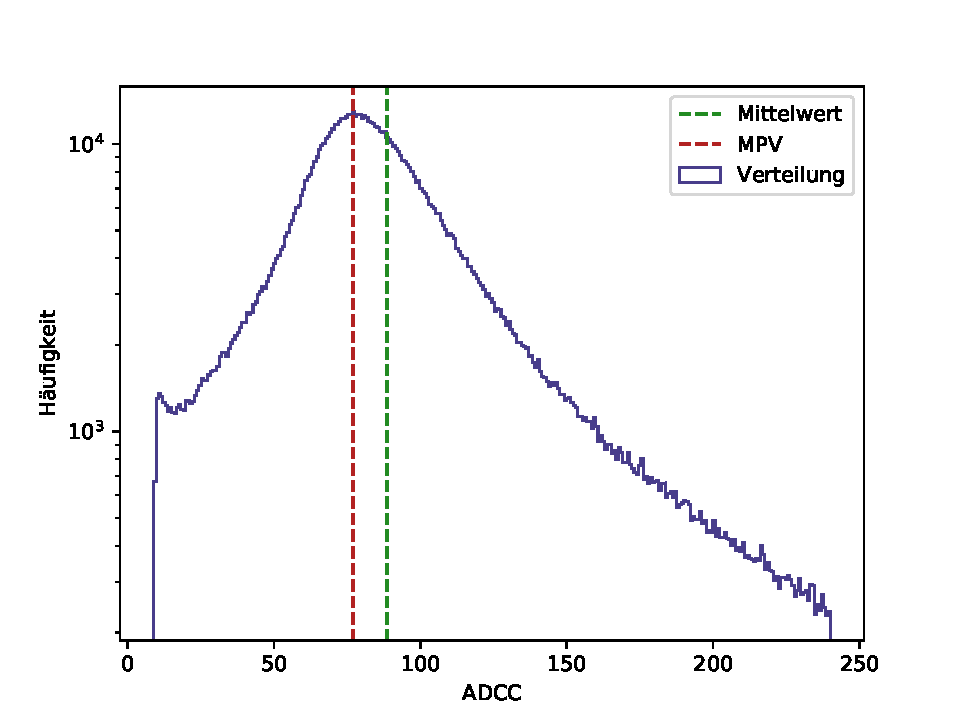
\includegraphics[width=0.8\textwidth]{plots/spectrum_adc.pdf}
  \caption{Energiespektrum der $^{90}$Sr-Quelle in der Einheit ADCC.}
  \label{fig:spektrumADCC}
\end{figure}

\begin{figure}
  \centering
  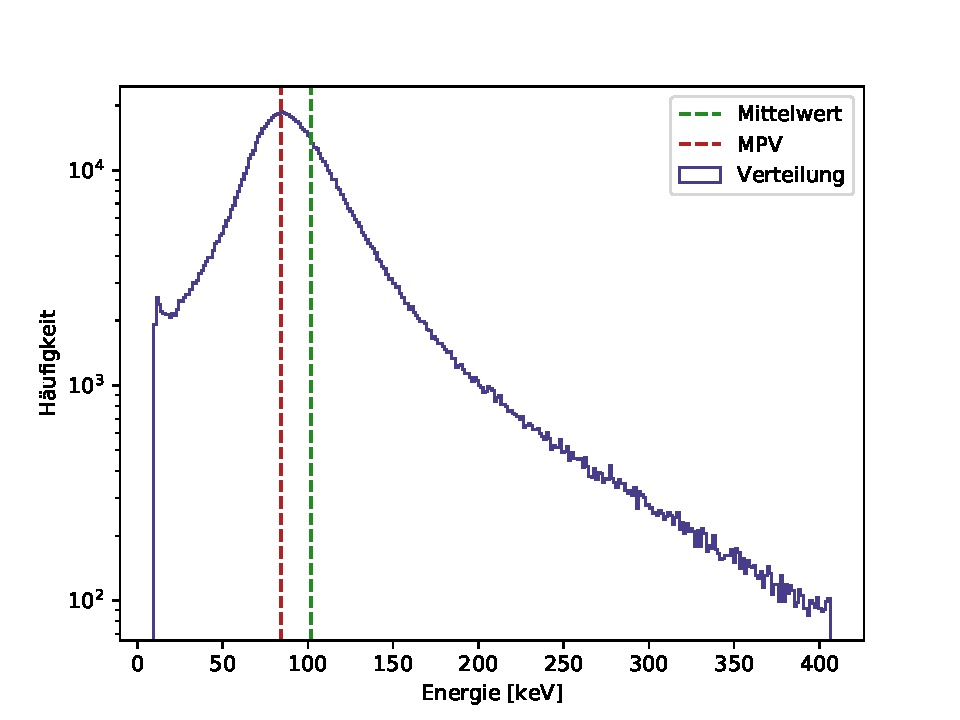
\includegraphics[width=0.8\textwidth]{plots/spectrum_keV.pdf}
  \caption{Energiespektrum der $^{90}$Sr-Quelle in der Einheit keV.}
  \label{fig:spektrumkeV}
\end{figure}
\FloatBarrier

Aus den Spektren wird ein Mittelwert von
\begin{align*}
  \bar{E} = \SI{88.65 \pm 0.04}{ADCC} = \SI{101.99 \pm 0.05}{\kilo\electronvolt}
\end{align*}
bestimmt, während über das Verteilungsmaximum der MPV zu
\begin{align*}
  MPV =  \SI{77 \pm 0.5}{ADCC} = \SI{84.0 \pm 1.0}{\kilo\electronvolt}
\end{align*}
ermittelt wird.
